\chapter{Fabrication of On-Chip Coplanar Waveguides}
\label{ch:Microfabrication}
For further investigation of spin transfer through the superconducting layer near and below the critical temperature, the next step was to fabricate a device capable of performing FMR on the samples while applying a DC current through the film, in order to modulate the damping \cite{Chen2024}. This required creating an isolation layer between the DC lines and the FMR lines, since the CPW needed to be fabricated directly on top of the sample, in order to achieve a strong signal. This chapter presents the methods investigated for creating an isolation layer via resist cross-linking, along with the final device fabrication process.

\section{Optimizing the cross-linking process}
The standard method for create such an isolation layer is through atomic layer deposition of a $SiO_2$ layer, however due to the technical difficulty of this process, an easier method was sought to achieve this. Cross-linking a resist was identified as promising. Several cross-linking techniques were investigated to determine the most effective approach for device fabrication, which are detailed in the following. These tests were done on silicon samples, as the substrate material is not expected to have a significant impact on the cross-linking process.
\subsection{Electron Beam Lithography}
The first attempts of cross-linking were done using EBL. For this, the $\textit{AR-N 1407.17 new}$ (AR-N) resist was spin-coated onto a silicon sample at 4000 rounds per minute (rpm) with an acceleration of 1000 rpm/s. The expected thickness was 40nm \cite{Allresist_ARN7520}. The sample was then soft-baked at 85 $^\circ$C for one minute and placed into the EBL. The electron beam was set to 20 kV and the aperture set to 20 µm, with a beam current of 112 pA.

To verify the concept, a small square on the sample with the side length of 100 µm was exposed with a dose of 10000 $\si{\micro C/cm^2}$, which was done by exposing the same area to 100 $\si{\micro C/cm^2}$ a hundred times. For reference, the dose recommended by the manufacturer is 30 $\si{\micro C/cm^2}$ \cite{Allresist_ARN7520}. After the overexposure, the sample was developed with the $\textit{AR300-47}$ developer for 50 seconds, and was submerged into deionized water for 30 seconds.

Following the development, a series of stress tests were done to mimic the real fabrication process, which included applying a pressurized stream of acetone onto the sample, submerging the sample into a acetone bath at 60$^\circ$C for 10 minutes. Subsequently, the sample was submerged in the $AZ351B$ developer for two minutes. Finally, the sample was put into an ultrasonic acetone bath at the highest setting (9/9) for one minute. In the actual sample, ultrasonic bath is potentially needed for the process of gold lift-off, where the lowest setting (1/9) is typically used.

The sample withstood the acetone stream well, although changes in color were visible after the acetone bath and the development step. The ultrasonic acetone bath removed only the unsuccessfully exposed regions, indicating that the cross-linking was successful and robust. However, the exposure took around three hours, which is long given the size of the exposed area. Since the target area on the final sample was significantly larger, it was considered critical to reduce the exposure time.

This led to an investigation of the minimal dose required to achieve sufficient cross-linking. Various areas of the sample were exposed to different doses, as shown in Figure \ref{fig:dose-exposure}. The exposure was applied in increments of 100 µC/cm$^2$ per layer.

\begin{figure}
    \centering
    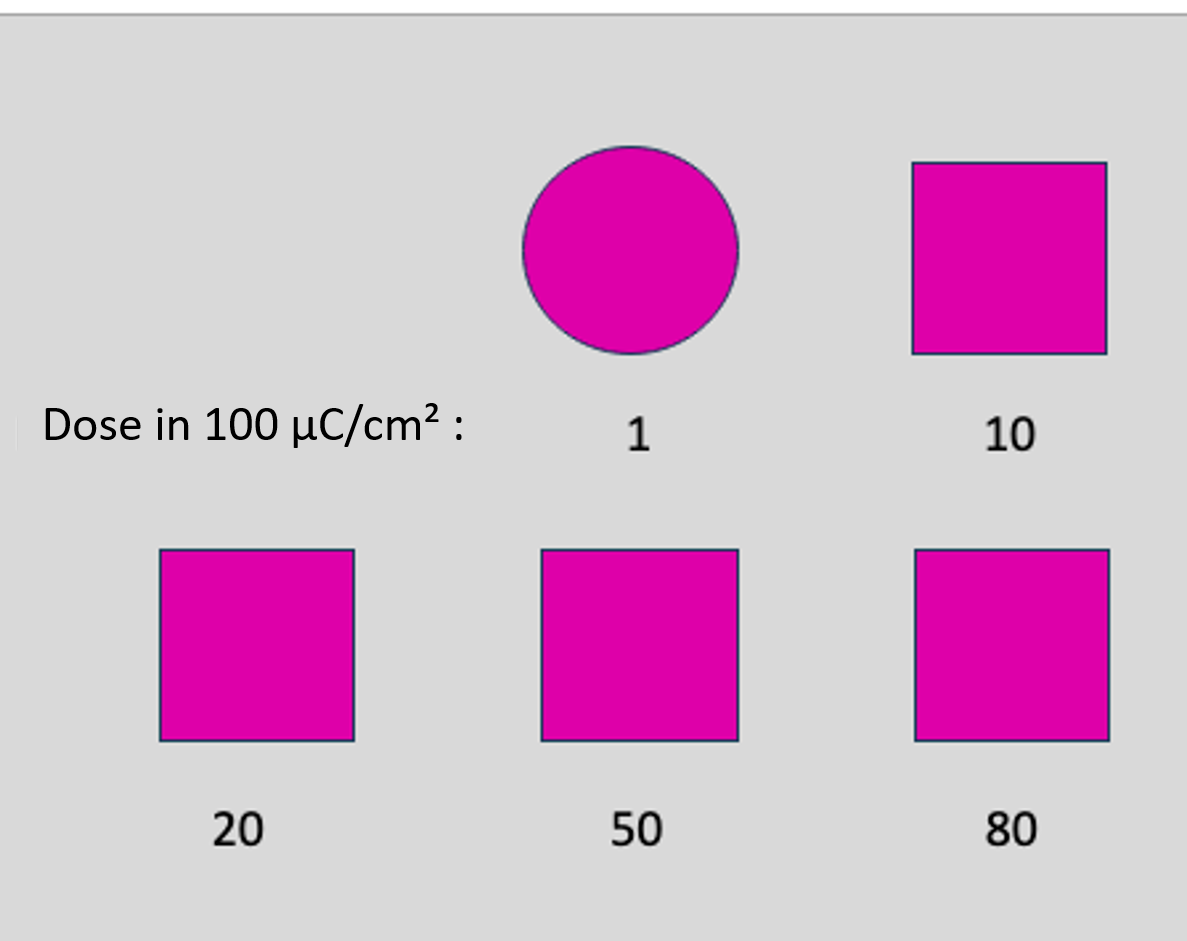
\includegraphics[width=0.6\linewidth]{chapters/Photos/Microfabrication/E-line Dose_corrected.png}
    \caption{Sample illustration of the exposure done with the EBL. The first exposed area is a circle for better orientation. The exposure was done in layers of 100 $\si{\micro C/cm^2}$.}
    \label{fig:dose-exposure}
\end{figure}

After the exposure, the sample was developed with the $\textit{AR300-47}$ developer for around two minutes, followed by a 30 second submersion in deionized water. The sample then underwent the same stress tests as before.
Some color changes were visible in the areas exposed with one to 20 layers of 100 $\si{\micro C/cm^2}$ after the acetone pressure stream, and the acetone bath seemed to make the area with 50 layers appear brighter. The $\textit{AZ351B}$ developer seemed to have no effect on the sample, but the ultrasonic fully removed the area exposed only once, as well as corroded the areas with 10 and 20 layers at the edges slightly.
Each exposed area was inspected with a microscope and the surface-roughness was investigated with an atomic-force microscope (AFM). In the end, it was concluded that a dose of 2000 $\si{\micro C/cm^2}$ (20 layers) was a good compromise between exposure time and durability. The corroded edges were deemed acceptable for the actual sample, as they would not impair the performance of the device in the center of the structure.

With this dose, the exposure on a real sample was estimated to take around 15 hours. However, during the actual attempt, the EBL shut down after seven hours. The exact cause remains unknown, though the most likely explanation is the combination of a large aperture and high beam current applied over a long time. Since the design to be exposed was relatively large, an aperture of 60 µm was chosen, resulting in a beam current of 1113 pA. The long duration may have led to overheating of the cathode.

Given these issues, it was attempted to scan the sample with the EBL without proper exposure of the design. For this, three corners of a sample coated with the AR-N resist were scanned with the EBL for 1, 5, and 10 minutes, respectively (denoted A, B, and C). The sample was then subjected to a stress test using an acetone bath followed by the $\textit{AR300-47}$ developer. Corner A was removed immediately in the acetone bath. Corner B remained visible after the bath, although significant damage was observed under the microscope (Figure \ref{fig:5min}).
\begin{figure}[htbp] % [htbp] for flexible placement
    \centering % Center the entire figure
    \begin{subfigure}[c]{0.48\textwidth} 
        \subcaption{Before acetone bath} % Place (a) above the image
        \centering
        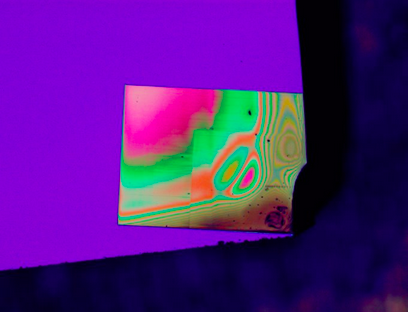
\includegraphics[width=\linewidth,height = 6cm]{chapters/Photos/Microfabrication/5min_before.png}
        \label{fig:5min_before}
    \end{subfigure}
    \hfill % Flexible horizontal space
    \begin{subfigure}[c]{0.48\textwidth} 
        \subcaption{After acetone bath} % Place (b) above the image
        \centering

        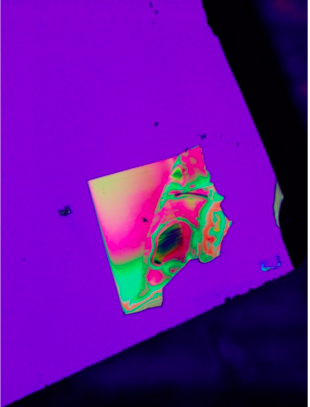
\includegraphics[width=\linewidth, height = 6cm]{chapters/Photos/Microfabrication/5min_after.png} 
        \label{fig:5min_after}
    \end{subfigure}
    \hfill % Flexible horizontal space
    \caption{Microscope images of the corner exposed for five minutes, before (a) and after (b) the acetone bath.}
    \label{fig:5min} % Main label for the entire figure
\end{figure}
Corner C was still intact after the acetone bath and the developer, but variances in color were visible, pointing to a thickness variance. The pictures taken under the microscope are shown in figure \ref{fig:10min}. Although the damage was less severe than in Corner B, it was still deemed substantial. Additionally, the high thickness variance would impair the performance of the device. The EBL was therefore deemed unfit for the fabrication of the isolation layer.
\begin{figure}
    % I want three pictures in one row
    \centering
    \begin{subfigure}[c]{0.32\textwidth} 
        \subcaption{Before acetone bath} % Place (a) above the image
        \centering
        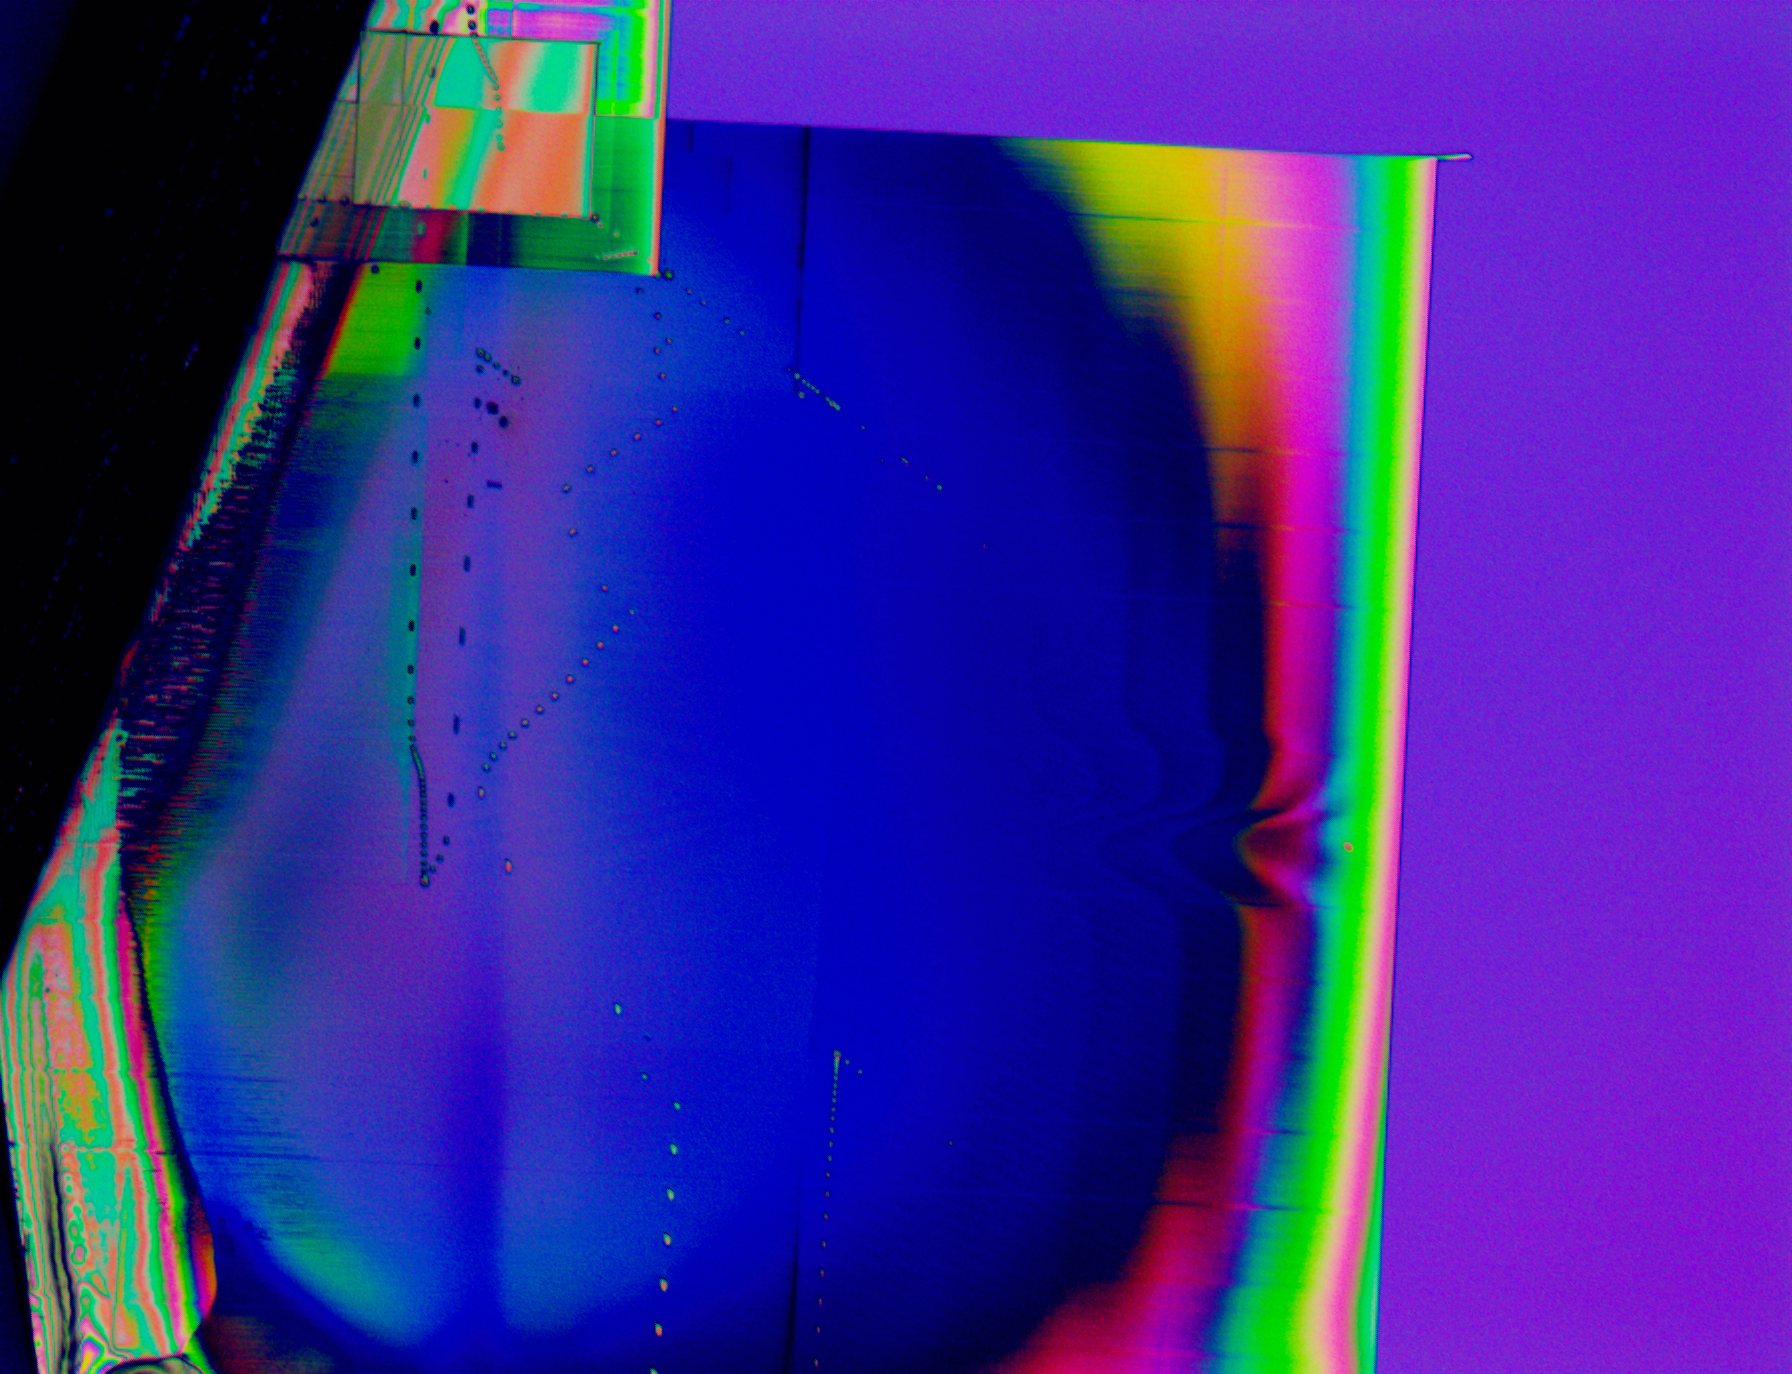
\includegraphics[width=\linewidth]{chapters/Photos/Microfabrication/10min_looking_ebeam.png}
        \label{fig:10min_before}
    \end{subfigure}
    \hfill % Flexible horizontal space
    \begin{subfigure}[c]{0.32\textwidth} 
        \subcaption{After acetone bath} % Place (b) above the image
        \centering
        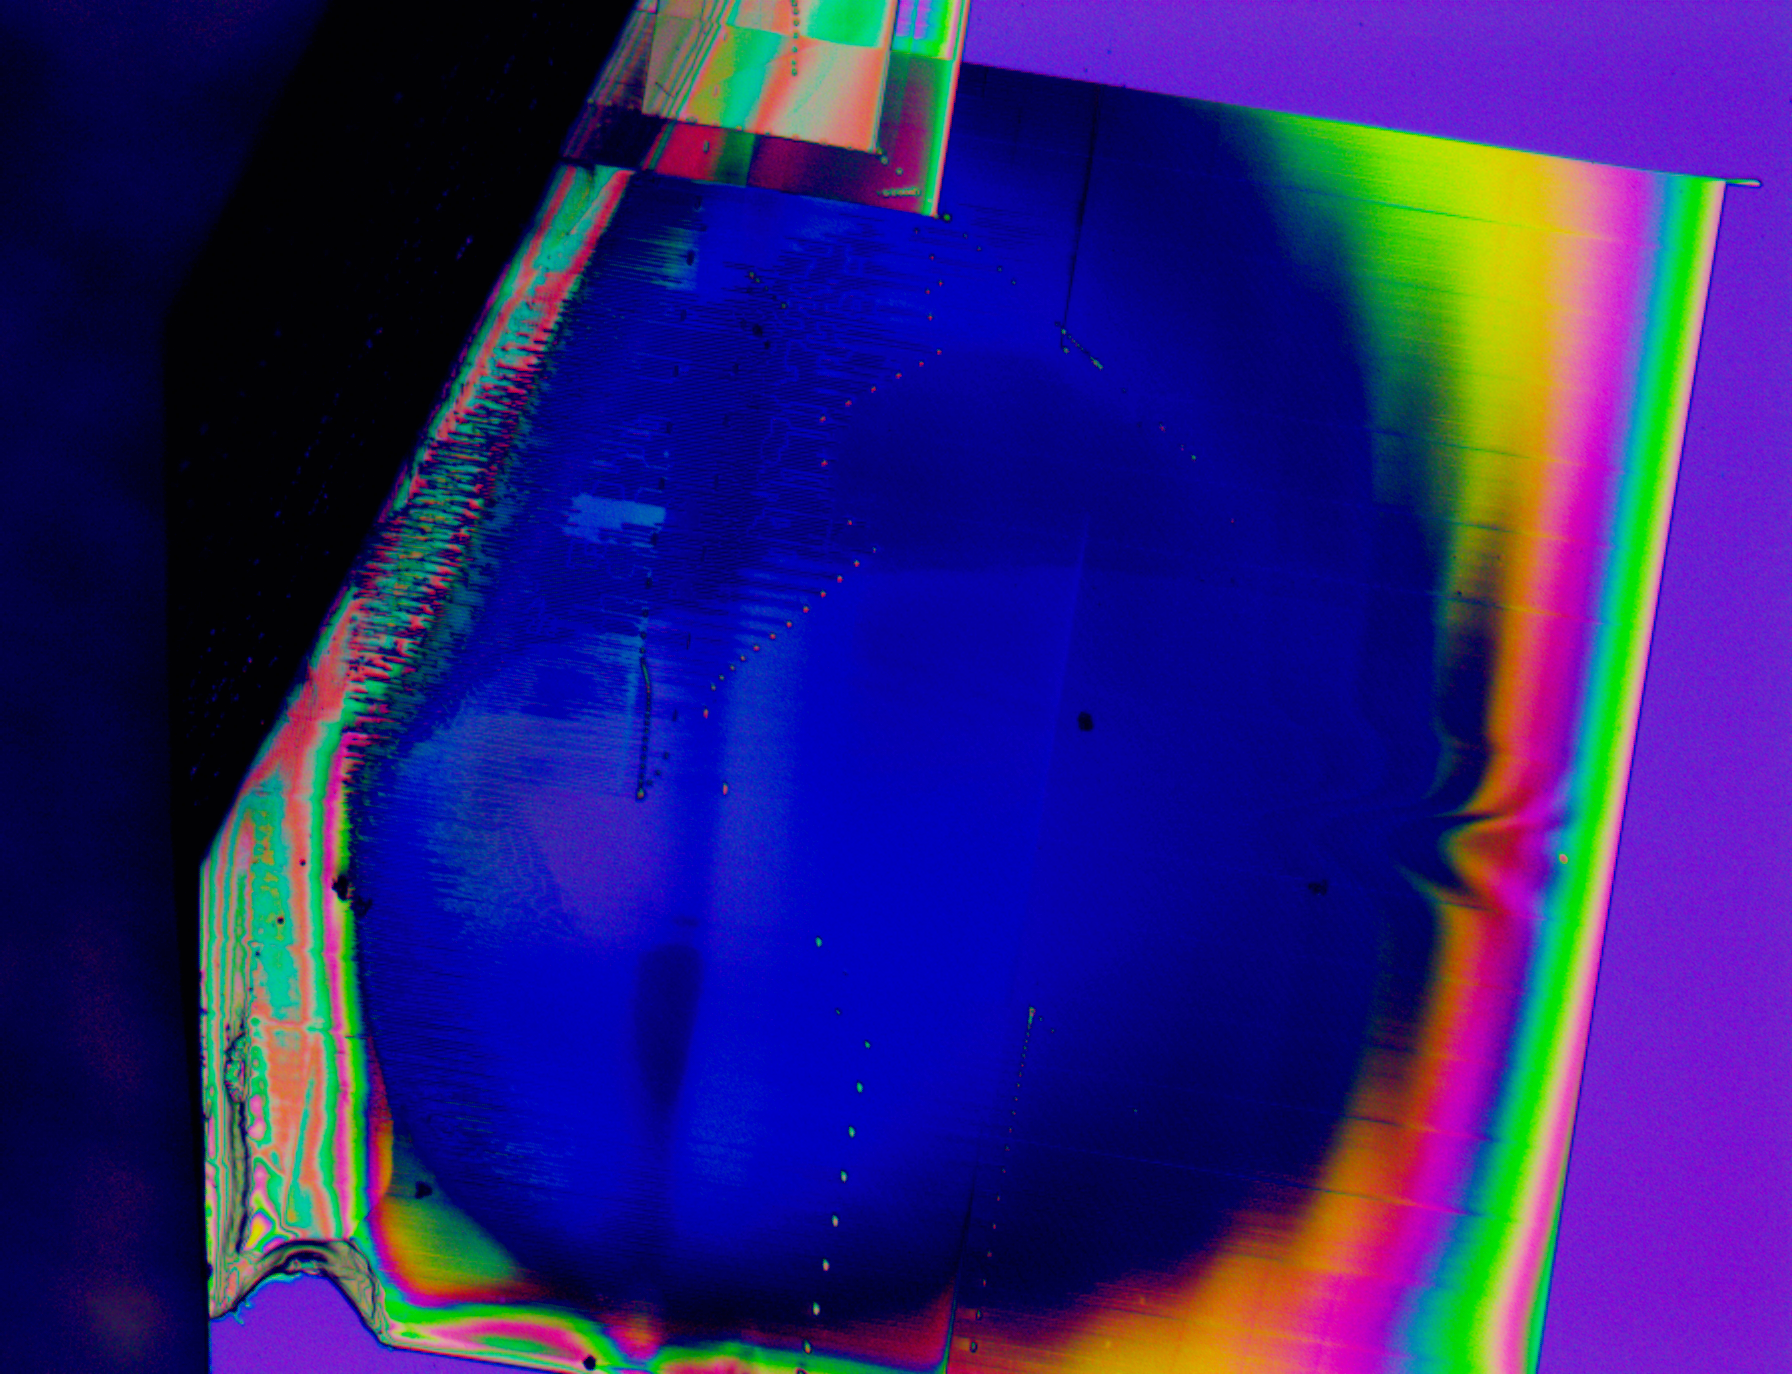
\includegraphics[width=\linewidth]{chapters/Photos/Microfabrication/10min_looking_ebeam_after_bath.png} 
        \label{fig:10min_after_bath}
    \end{subfigure}
    \hfill % Flexible horizontal space
    \begin{subfigure}[c]{0.32\textwidth} 
        \subcaption{After acetone bath + developer} % Place (c) above the image
        \centering
        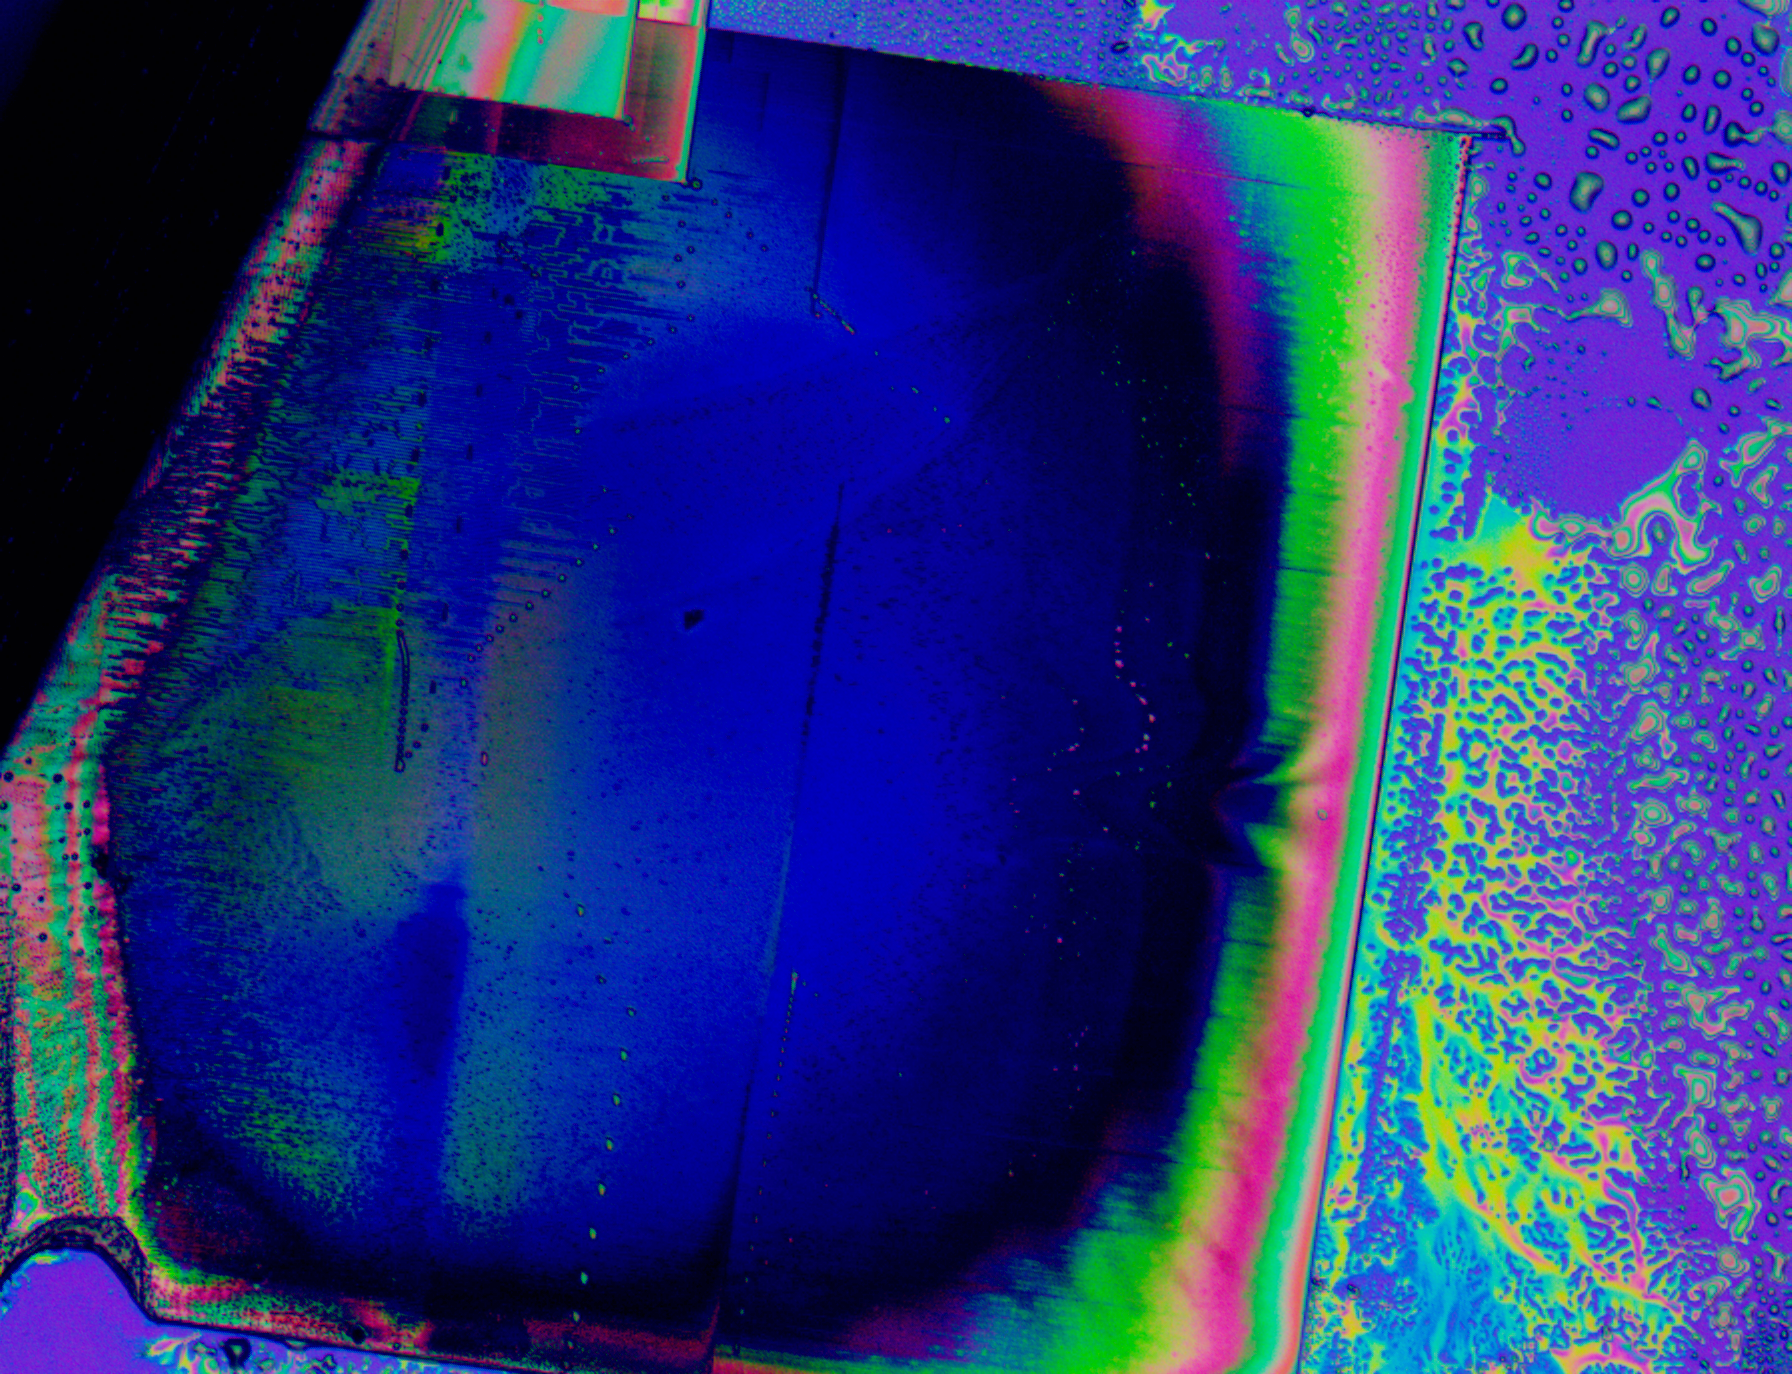
\includegraphics[width=\linewidth]{chapters/Photos/Microfabrication/10min_looking_ebeam_after_bath_and_dev.png} 
        \label{fig:10min_after_dev} 
    \end{subfigure}
    \hfill % Flexible horizontal space
    \caption{Image of the corner of the sample that was exposed for 10 minutes. There are certain spots visible that changed its color in (c).}
    \label{fig:10min} % Main label for the entire figure
\end{figure}

\subsection{Optical Lithography} 
\label{sec:Optical Lithography}
Instead of EBL, overexposure by photolithography can also be facilitated to cross-link resists. The AR-N resist is an e-beam resist, meaning it is best suited for use with an EBL machine, but it is also reactive to deep UV light (248-365 nm) \cite{Allresist_ARN7520}. The resist was spin-coated onto a silicon sample and exposed to various spots with different doses, using a MLA. Doses from 800-2300 $\si{\micro C/cm^2}$ were tested to investigate the optimal exposure conditions.
After the exposure, the sample underwent the same stress test procedure as the samples exposed with the EBL to investigate its chemical tolerance against the steps that the actual isolation layer will need to withstand. After the acetone stream, some spots were visible on some dose. The acetone bath seemed to have some effect, especially on the lower doses, but the sample was still intact for the higher doses. The ultrasonic bath was omitted, however.

This method showed great durability and seemed to be able to withstand the stress test, even at a dose of 1000 $\si{\micro C/cm^2}$. However, there were multiple stripes visible on the sample at all doses, which pointed to a high variance in thickness. The stripes were caused by the MLA exposing small areas (write fields) one at a time. When moving from one write field to another, the edge can be exposed multiple times, leading to variations in thickness. An AFM was used to investigate the thickness of the resist and the stripe topography, which is shown in figure \ref{AFM_MLA}.

\begin{figure}
    \centering
    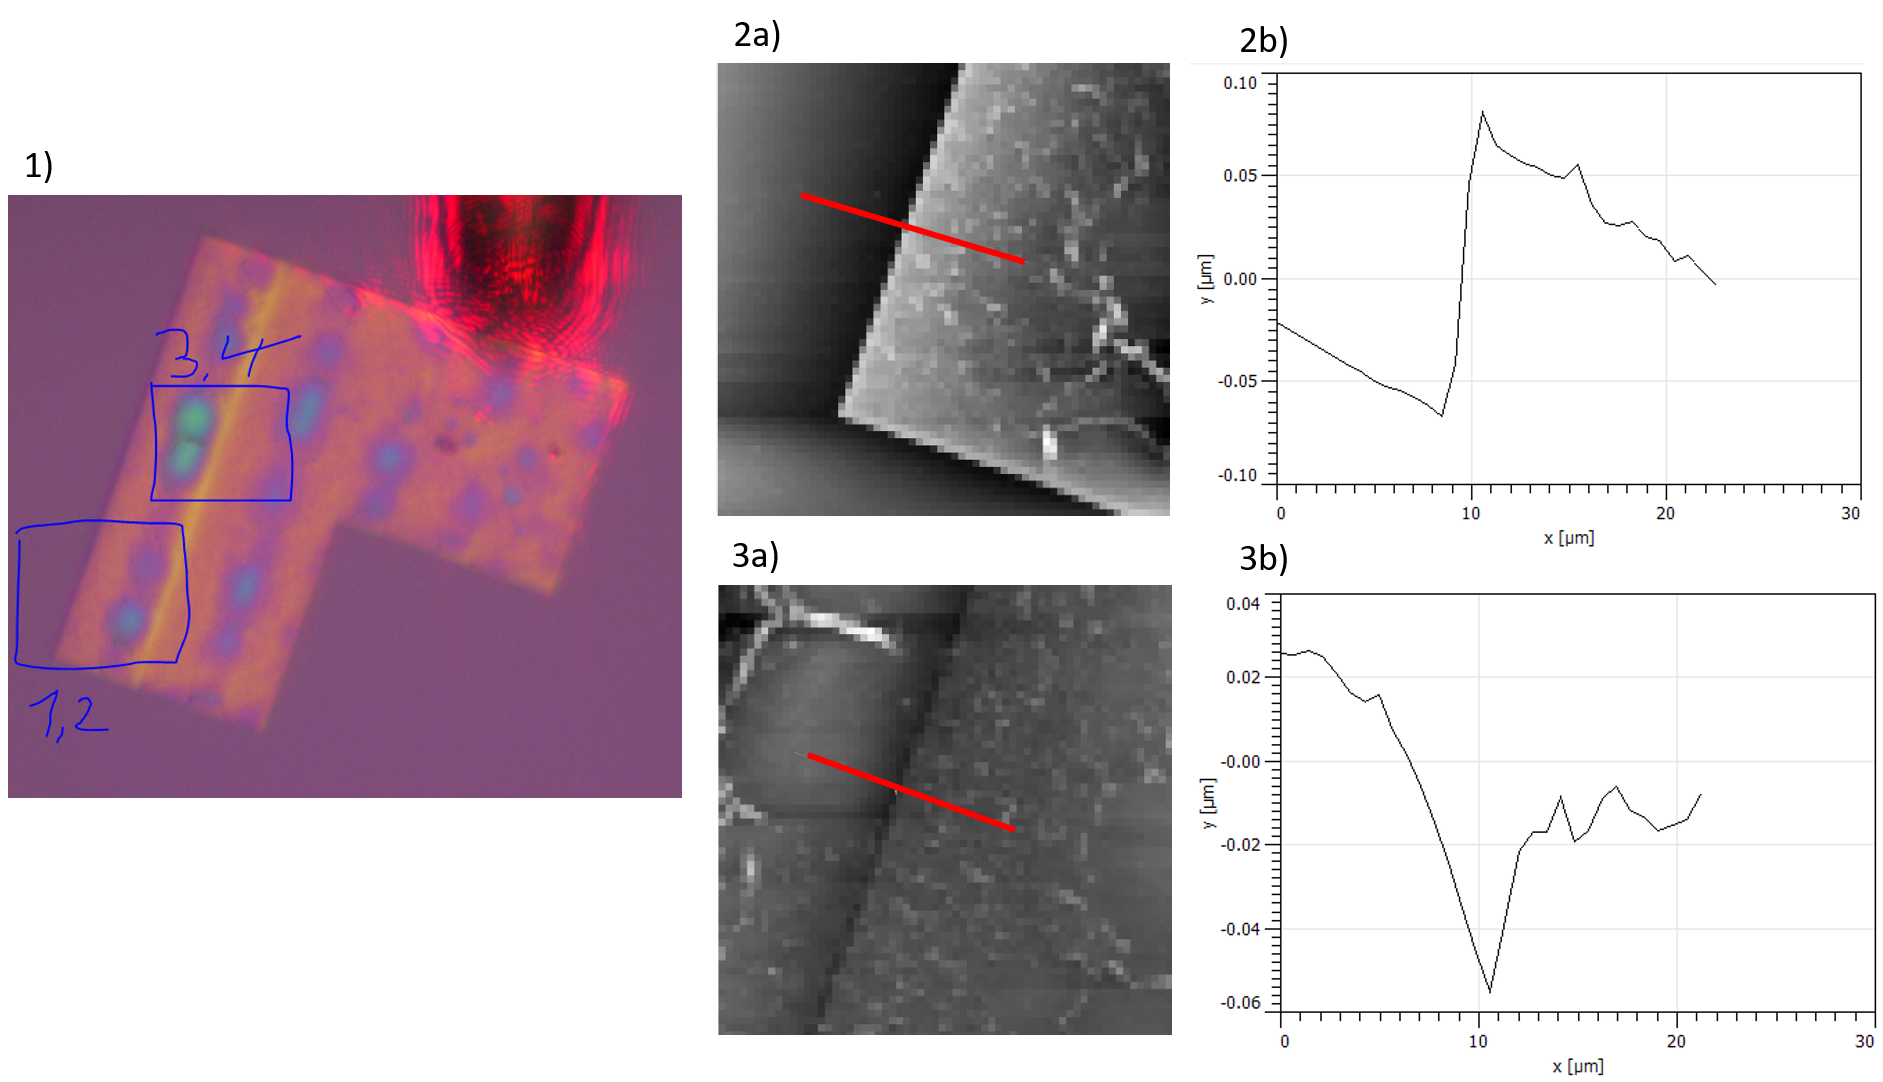
\includegraphics[width=\linewidth]{chapters/Photos/Microfabrication/test2.png}
    \caption{AFM measurement of the resist thickness after MLA exposure. The pictures 2a and 2b correspond to the area marked as (1,2) in picture 1. Similarly, the pictures 3a and 3b correspond to the area marked as (3,4) in picture 1.}
    \label{AFM_MLA}
\end{figure}

The AFM measurements revealed a significant variance in the thickness of the resist across the sample. The resist had an overall thickness of around 140 nm (which can be seen from picture 2b in figure \ref{AFM_MLA}). The stripes, however, were more than 70nm in height. This could lead to problems such as a non-even CPW, which would affect the RF transmission of the device.

After the AFM measurement, it was tried dividing the exposure into multiple steps and rotating the sample between the steps to even out the stripe. This, however, showed no significant improvement. This method was therefore deemed unfit for the isolation layer, as the variance in thickness would lead to an uneven surface. Another researcher at the chair (Samuel Fülop), however, found out after the conclusion of this work that the issue with the stripes can be resolved by applying a significantly higher dose of 45000 $\si{\micro C/cm^2}$, which is the main way isolation layers are now fabricated at the chair.
\subsection{Overexposure by an incoherent light source}
To avoid stripes, it was investigated whether exposing the resist globally with a light source of a microscope would be a viable option. For this, the $\textit{MA-N 1407}$ (MA-N) resist was used, which was spin-coated onto a silicon sample, followed by a softbake at 100C$^\circ$ for 5 minutes. The sample was then exposed with a microscope for 10min at the lowest magnfication such that the entire sample was evenly illuminated by the light source. After the exposure, the sample was developed with the $\textit{ma-D 533/S}$ developer for 25 seconds and put into deionized water for 30 seconds. Subsequently, an acetone stream was applied onto the sample. The sample did not withstand the process and the resist washed away completely. This method was therefore considered unfit for the isolation layer.

\subsection{Overbaking}
Finally, it was investigated whether overbaking the resist, as in doing the pre-baking process significantly longer than recommended, would lead to a durable isolation layer.
For this, samples were spincoated with both the AR-N and the MA-N resist onto silicon samples at their respective recommended rpm settings, which are detailed in the sections above. The samples were then put onto a hotplate at 100C$^\circ$ for 20 minutes to overbake them.

Both samples then underwent stress tests which included pressurized acetone streams, submersion in their respective developer, and acetone baths. The overbaked sample with the AR-N resist was damaged after the test.
The sample with the MA-N resist, however, withstood the stress test and and stayed in tact after an acetone bath of 10 minutes, although there were some holes visible in the isolation layer, which are shown in figure \ref{holes}. The holes were deemed acceptable, as they would be covered by the gold layer of the CPW during the actual fabrication process and would not be exposed to the chemical used during the stress test except the developer, which did not seem to have an effect on the sample.

\begin{figure}
        \centering
        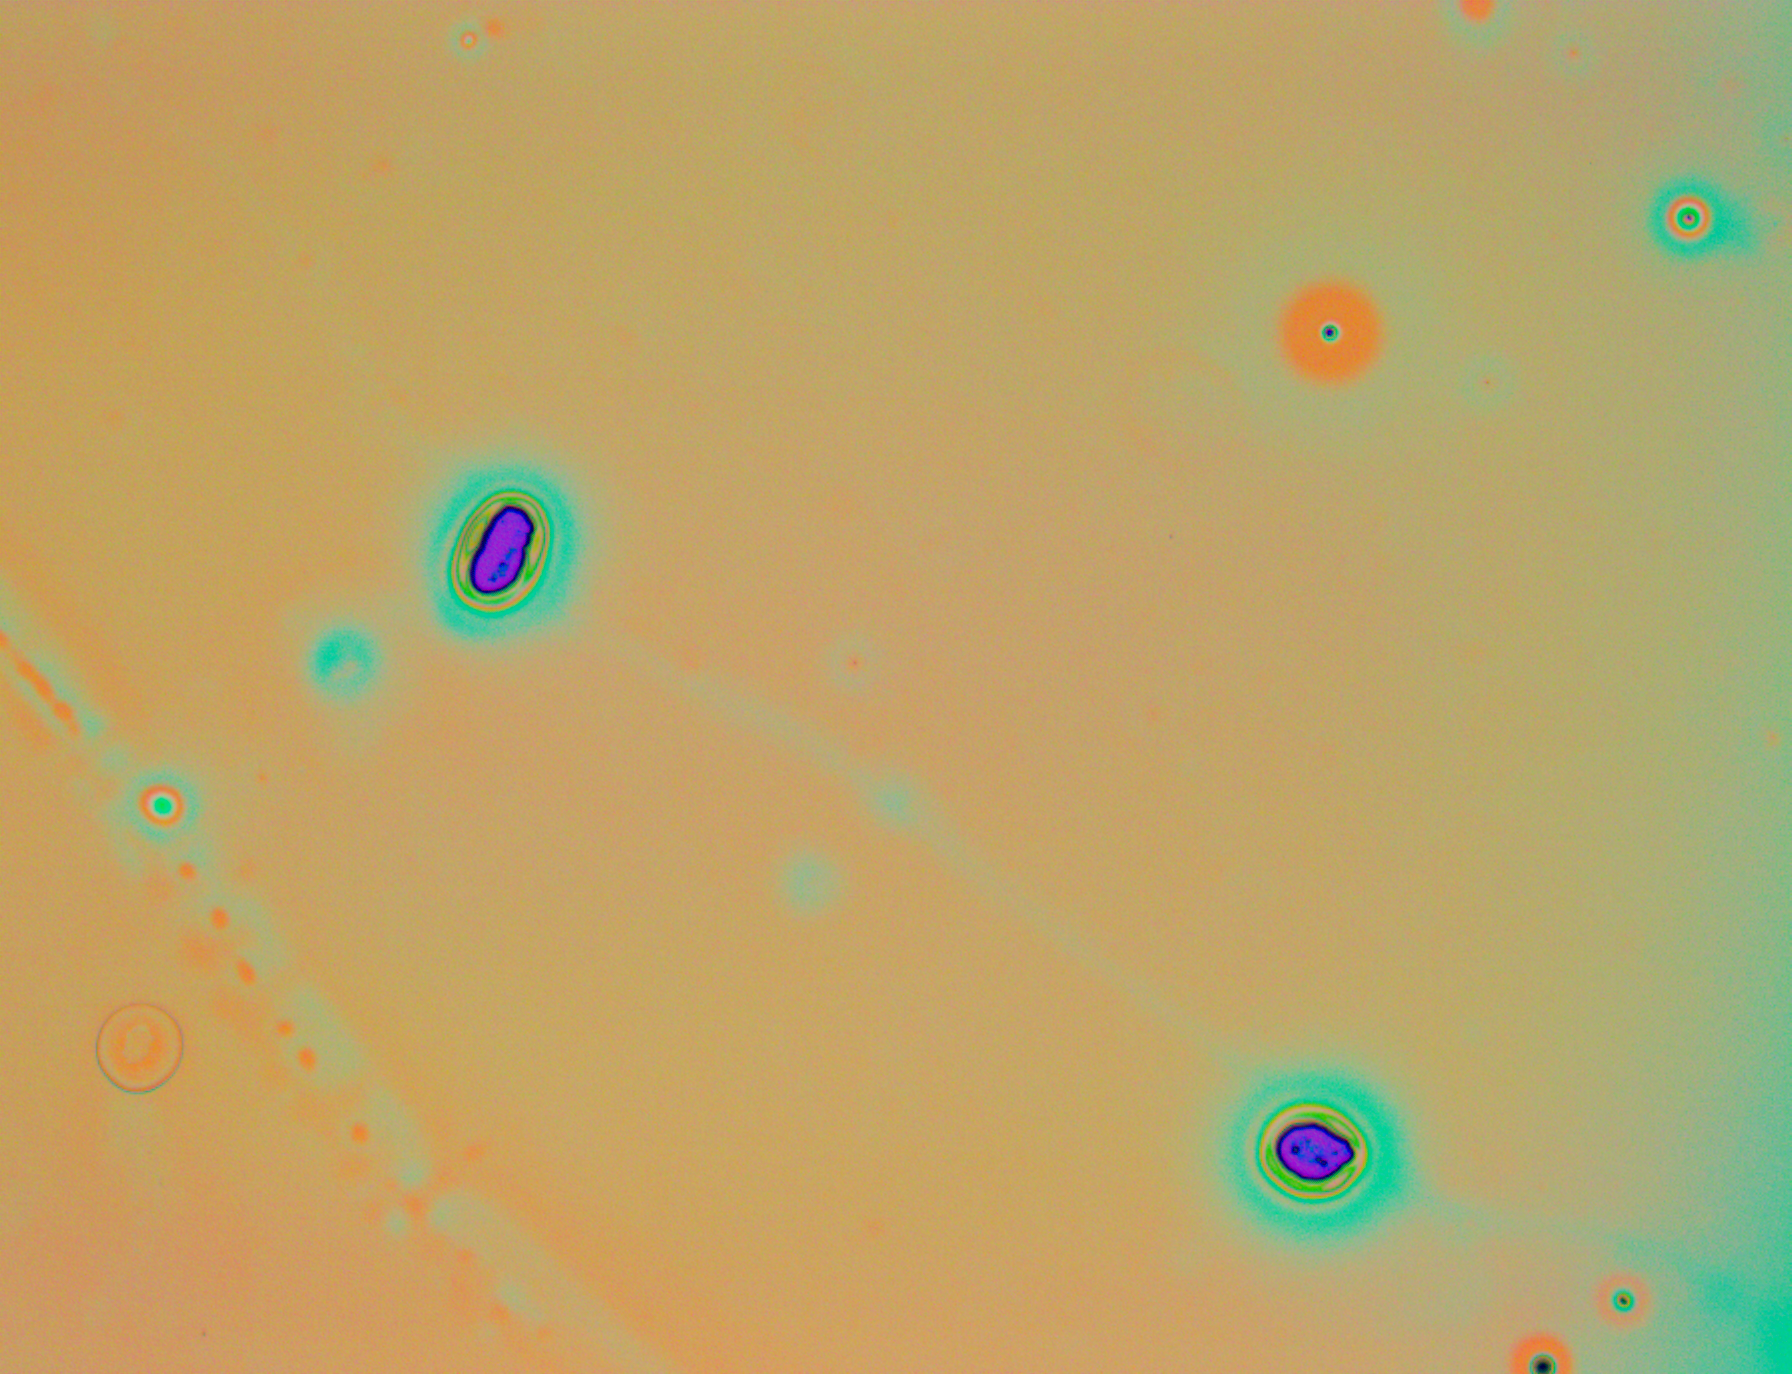
\includegraphics[width=0.7\linewidth]{chapters/Photos/Microfabrication/MaN_holes.png}
        \caption{Picture of the holes seen in the isolation layer of the overbaked sample with the $\textit{MA-N 1407}$ resist. The sample was overbaked at 100$^\circ$C for 20 minutes, and then underwent a stress test which included an acetone bath for 10 minutes.}
        \label{holes}
    \end{figure}

\section{Fabrication of on-chip waveguides}
In order to test the isolating functionality on a real device, the overbaking process was first used to fabricate on-chip waveguides, as it was found to be a promising method, having an even surface and no significant defects. After Fülop found that the MLA can be used for even better results (see section \ref{sec:Optical Lithography}), the process was adapted accordingly. In the following, the entire process is explained by which a device capable of FMR measurements under a DC-bias was successfully fabricated using the overexposure method.

The full design can be taken from figure \ref{fig:design_sample}. The design at the bottom includes the CPW and the contact pads for electrical connections, as well as the isolation layer between them. 

\begin{figure}
    \centering
    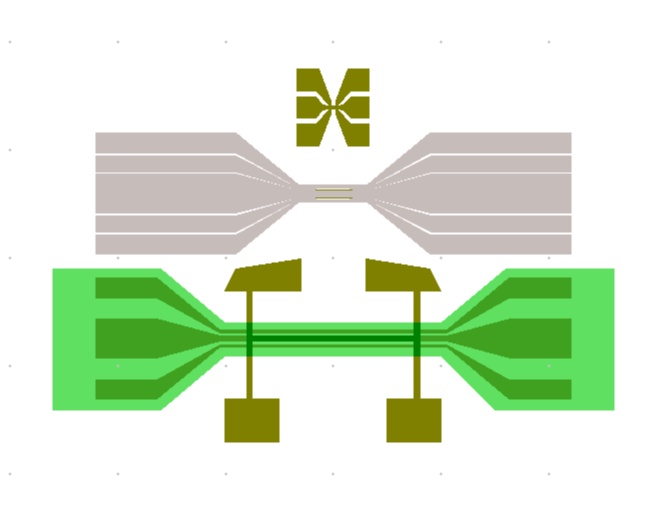
\includegraphics[width=0.8\textwidth]{chapters/Photos/Microfabrication/Design_Chip.PNG}
    \caption{Design of the device for FMR measurements. The design at the bottom includes the CPW (gold on the green layer) and the contact pads for electrical connections (gold), as well as the isolation layer (green) between them.}
    \label{fig:design_sample}
\end{figure}

\subsection{Fabrication}
Firstly, a full-film sample is spin-coated with the Ma-N resist, after which it is soft-baked at 100 C$^\circ$ for 1 minute. The sample is then placed into the MLA and the mesa layer is exposed. After developing, the sample undergoes a pre-sputtering of 10 minutes to remove the film at the non-exposed areas.
After the etching and removing the residual resist, the sample is again spin-coated with the Ma-N resist and exposed with the MLA with a dose of 45000 $\si{\micro C/cm^2}$ to create the isolation layer needed.
Following the cross-linking step, the sample is now spin-coated with the $\textit{AZ 5214 E}$ (AZ) resist, which is a positive resist, and then soft-baked at 100 C$^\circ$ for 3 minutes. The contact pad and CPW layer is then exposed using the MLA. After exposure, the sample was etched again for 30 seconds to clean the surface, followed by evaporation of gold onto the sample for a thickness of around 100 nm. The sample is then put into an ultrasonic acetone bath at the lowest setting (1/9) for 30 seconds to remove the resist and lift off the gold from the non-exposed areas. The final sample is shown in figure \ref{final_sample}. It is clearly visible that the mesa layer is below the green isolation layer. The CPW flows over the isolation layer, indicating a successful fabrication process.

\begin{figure}
    \centering
    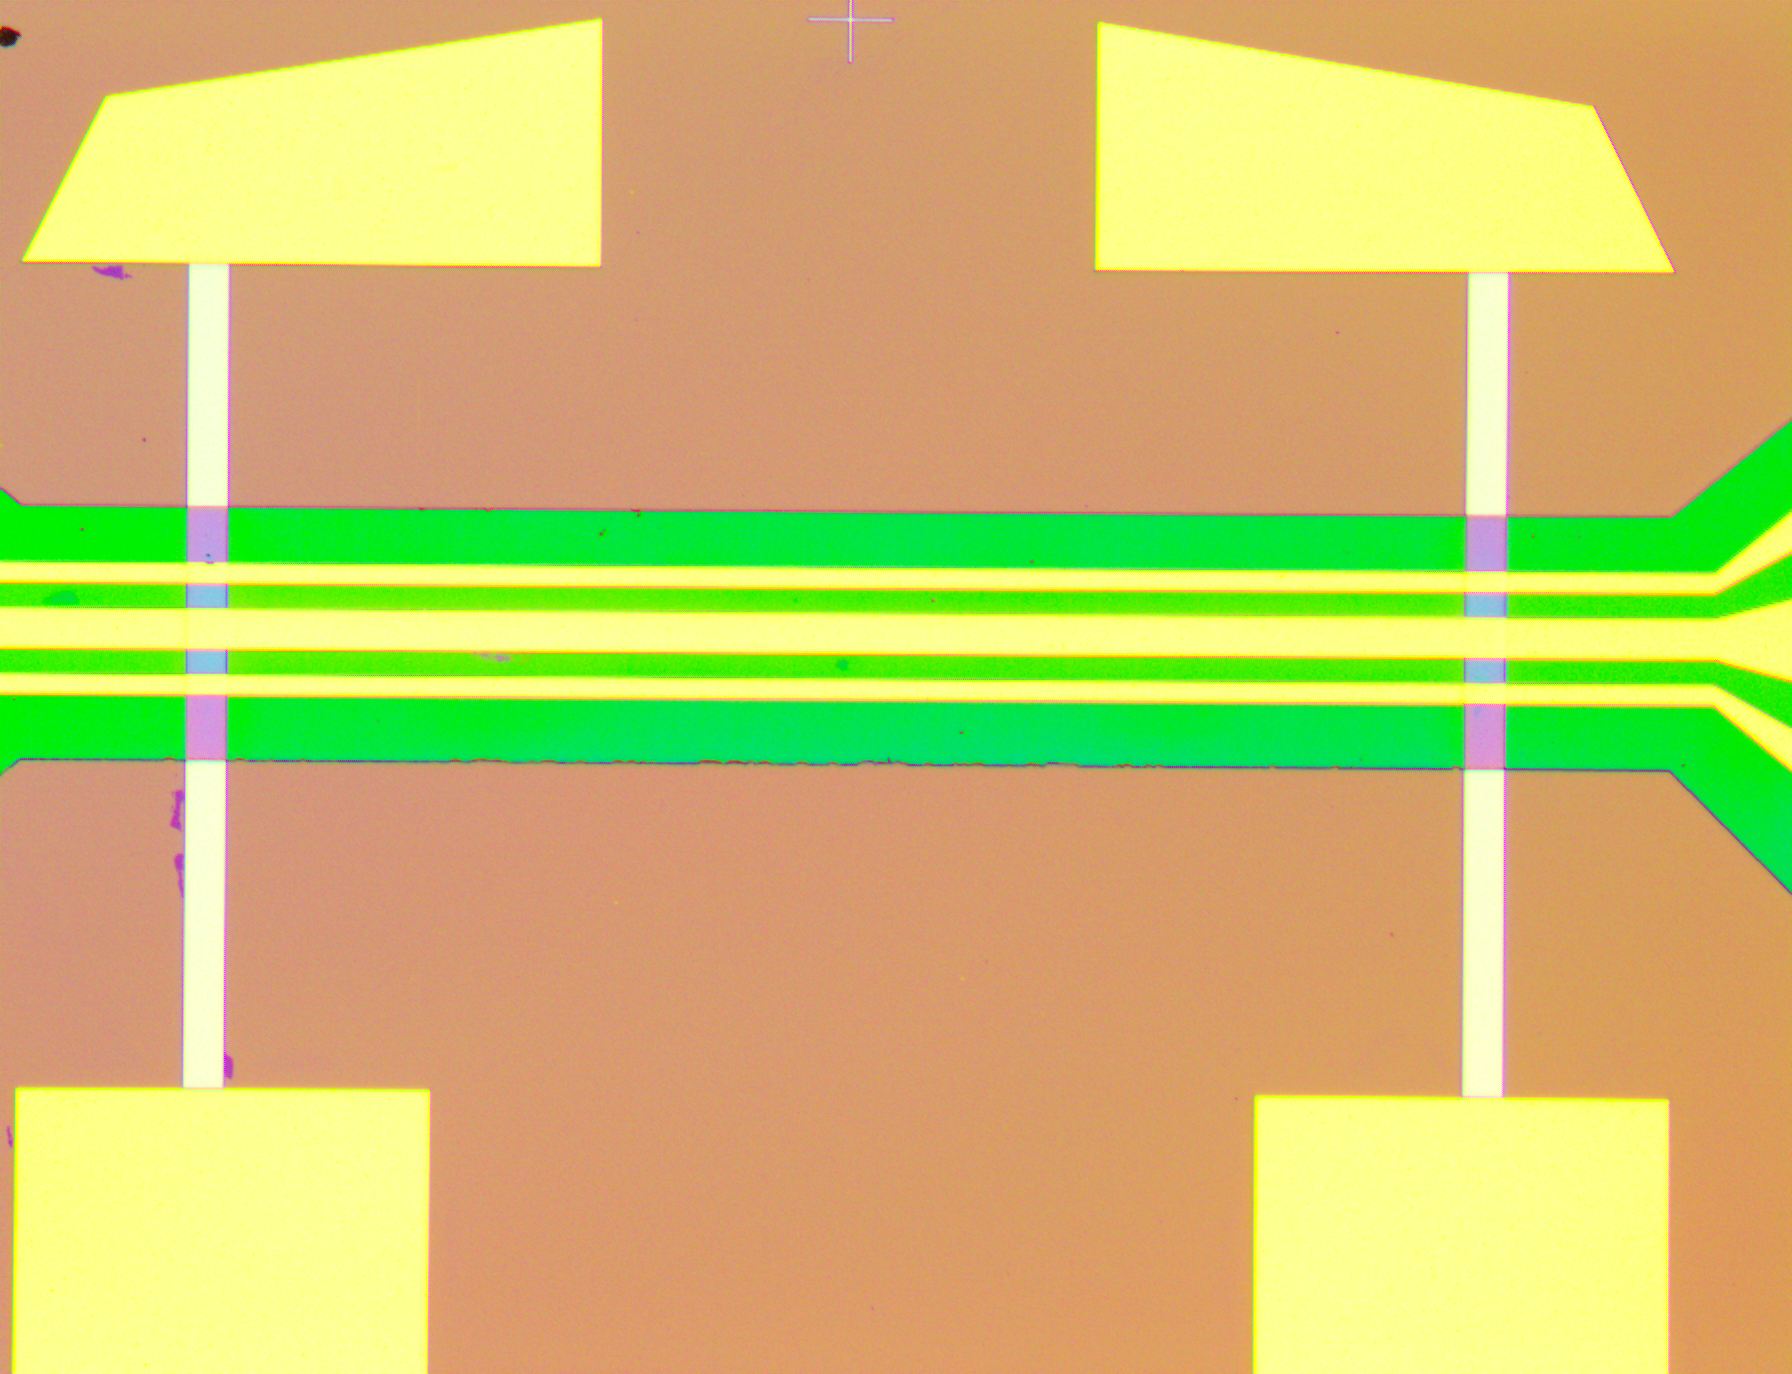
\includegraphics[width=0.7\textwidth]{chapters/Photos/Microfabrication/final_sample.png}
    \caption{Final sample after the fabrication process. The four contacts pads are visible in the corners. The mesa layer is below the green isolation layer, with the CPW flowing over the isolation layer. Courtesy of Max Mangold.}
    \label{final_sample}
\end{figure}

The holes encountered during the initial test were again to be seen after the final fabrication process. Some holes unfortunately were created exactly on the lines of the CPW, which could potentially affect the performance of the device. However, due to the redundant design of the CPW, the impact on the overall functionality was minimal. For initial test measurements, the CPW which was potentially compromised was simply not used.

\subsection{Soldering and bonding}
In order to mount the device into the insert for measurement, the signal and ground lines of the CPW are wire bonded to the transmission lines of the chip carrier, on which a SMA adapter is soldered. Additionally, wire bonds are done between the contact pads and other bond pads which are connected to a DC source. An example picture of a mounted device can be seen in figure \ref{fig:mounted_device}.

\begin{figure}
    \centering
    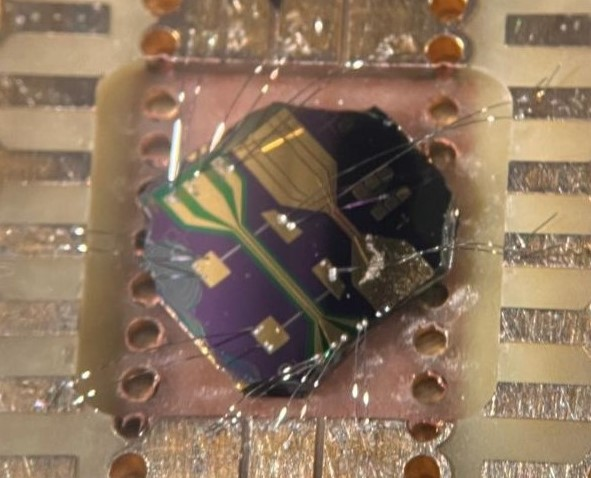
\includegraphics[width=0.7\textwidth]{chapters/Photos/Microfabrication/Mounted Device.jpg}
    \caption{Example of a device mounted onto the chip carrier. The wire bonds are done between the signal and ground lines of the CPW and the bond pads on the chip carrier, as well as between the contact pads and the bond pads connected to a DC source. All bonds were done twice for redundancy. The particular sample is mounted to achieve a 45° angle between the in-plane field and the DC current. Courtesy of Max Mangold.}
    \label{fig:mounted_device}
\end{figure}

\subsection{Testing of the device}
The testing of the fabricated device was carried out by Max Mangold using the FMR measurement setup described in chapter \ref{ch:Experimental Setup}.

The FMR measurement using the on-chip CPW was successful without any issues. The contact pads and the CPW seemed not have any shorting contacts, and a FMR signal was detected. However, the DC-bias does not seem to have an effect on the measurements on this sample as of now, other than warming up the sample at large currents. This is expected though, since any effects arising from spin-momentum coupling in the Nb and/or Pt layers on the Permalloy magnetization are expected to cancel out in symmetric stacks.


\subsection{Outlook}
During the course of this thesis, it was verified that cross-linking a resist can be done to create an isolation layer for fabricating a device capable of FMR measurements under a DC-bias. The method of overbaking was identified as a viable method. However, as stated above, Samuel Fülop found a more suitable method using the MLA. This is now the main method used at the chair for creating isolation layers via cross-linking, as it allows for local exposure.

As a next step, fabrication of the same device on asymmetric stacks are planned, to investigate the effect of DC currents and supercurrents on the Gilbert damping.



